\tikzstyle{init} = [pin edge={to-,thin,black}]
\tikzstyle{circ} = [circle, minimum size=1cm, text centered, draw=black, fill=blue!20]
\tikzstyle{arrow} = [thin,->,>=stealth]
\tikzstyle{arrow_t} = [very thin,->,>=stealth]

\tikzstyle{perc_in} = [circle, minimum size=1mm, text centered, draw=black, fill=blue!20]
\tikzstyle{perc_ou} = [circle, minimum size=1mm, text centered, draw=black, fill=red!20]
\tikzstyle{perc_hi} = [circle, minimum size=1mm, text centered, draw=black, fill=green!20]

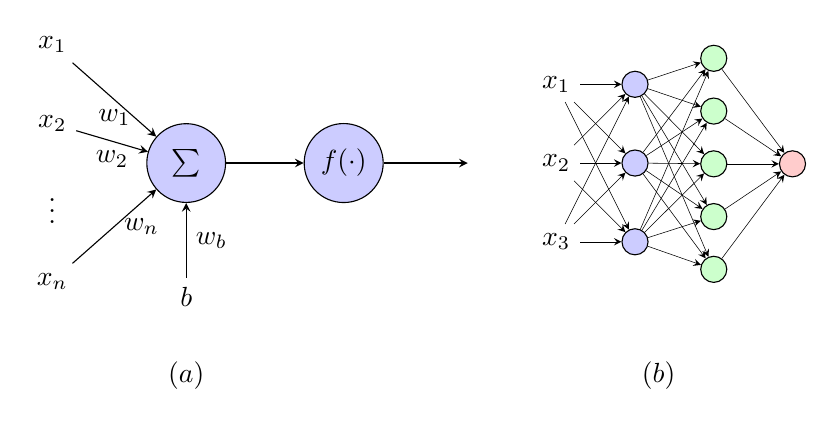
\begin{tikzpicture}
% Perceptron
\node (x1) [init] {$x_1$};
\node (x2) [init, below of=x1] {$x_2$};
\node (vdots) [init, below of=x2] {$\vdots$};
\node (xn) [init, below of=vdots] {$x_n$};

\node (sum) [circ, right of=x2, xshift=0.7cm, yshift=-5mm] {$\sum$};
\node (b) [init, below of=sum, yshift=-0.7cm] {$b$};
\node (obj) [circ, right of=sum, xshift=1cm] {$f(\cdot)$};
\node (output) [init, right of=obj, xshift=0.7cm] {};

\draw [arrow] (x1) --node[anchor=north] {$w_1$} (sum);
\draw [arrow] (x2) --node[anchor=north] {$w_2$} (sum);
\draw [arrow] (xn) --node[anchor=west] {$w_n$} (sum);
\draw [arrow] (b) --node[anchor=west] {$w_b$} (sum);
\draw [arrow] (sum) -- (obj);
\draw [arrow] (obj) -- (output);

% ANN
\node (i2) [init, right of=output] {$x_2$};
\node (i1) [init,, above of=i2] {$x_1$};
\node (i3) [init, below of=i2] {$x_3$};

\node (in0) [perc_in, right of=i1] {};
\node (in1) [perc_in, below of=in0] {};
\node (in2) [perc_in, below of=in1] {};

\node (hi0) [perc_hi, right of=in0, yshift=3.3mm] {};
\node (hi1) [perc_hi, below of=hi0, yshift=3.3mm] {};
\node (hi2) [perc_hi, below of=hi1, yshift=3.3mm] {};
\node (hi3) [perc_hi, below of=hi2, yshift=3.3mm] {};
\node (hi4) [perc_hi, below of=hi3, yshift=3.3mm] {};

\node (ou0) [perc_ou, right of=hi2] {};

\draw [arrow_t] (i1) -- (in0);
\draw [arrow_t] (i1) -- (in1);
\draw [arrow_t] (i1) -- (in2);
\draw [arrow_t] (i2) -- (in0);
\draw [arrow_t] (i2) -- (in1);
\draw [arrow_t] (i2) -- (in2);
\draw [arrow_t] (i3) -- (in0);
\draw [arrow_t] (i3) -- (in1);
\draw [arrow_t] (i3) -- (in2);

\draw [arrow_t] (in0) -- (hi0);
\draw [arrow_t] (in0) -- (hi1);
\draw [arrow_t] (in0) -- (hi2);
\draw [arrow_t] (in0) -- (hi3);
\draw [arrow_t] (in0) -- (hi4);
\draw [arrow_t] (in1) -- (hi0);
\draw [arrow_t] (in1) -- (hi1);
\draw [arrow_t] (in1) -- (hi2);
\draw [arrow_t] (in1) -- (hi3);
\draw [arrow_t] (in1) -- (hi4);
\draw [arrow_t] (in2) -- (hi0);
\draw [arrow_t] (in2) -- (hi1);
\draw [arrow_t] (in2) -- (hi2);
\draw [arrow_t] (in2) -- (hi3);
\draw [arrow_t] (in2) -- (hi4);

\draw [arrow_t] (hi0) -- (ou0);
\draw [arrow_t] (hi1) -- (ou0);
\draw [arrow_t] (hi2) -- (ou0);
\draw [arrow_t] (hi3) -- (ou0);
\draw [arrow_t] (hi4) -- (ou0);

\node (label_a) [init, below of=b] {$(a)$};
\node (label_a) [init, right of=label_a, xshift=5cm] {$(b)$};
\end{tikzpicture}